% ---------------------------------------------------
% ----- Chapters of the template
% ----- for Bachelor-, Master thesis and class papers
% ---------------------------------------------------
%  Created by C. Müller-Birn on 2012-08-17, CC-BY-SA 3.0.
%  Freie Universität Berlin, Institute of Computer Science, Human Centered Computing. 
%
\chapter{Theoretical background}

This thesis can be divided into two mayor areas of theoretical background.
Human-Computer-Interaction (HCI) and project specific background.

\section{HCI}
Let me start by explaining the HCI aspects and why this thesis approaches the area from an not so common standpoint.
\\
Many HCI books (e.g. \cite{Interactiondesign:2019ys} or \cite{LearnHCI:2020ys}) implicitly assume \label{def:Greenfield} Greenfield development,
which ''[...] is in its most distinct form when a new product is created from scratch – a new product or product platform, based on new technology, using new methodology and implemented by people who are new to it all.'' \cite{BrownfieldToGreenfield:2021ys}.
\\
While they mention \textit{Environmental requirements} as part of the requirement discovery, this usually is more focused on what abilities the users have (TODO), and not on the restrictions imposed by older software companies, especially those colloquially called ''enterprise''.

There, besides the omnipresent time and capacity restrictions and sometimes not that constructive inputs from stake holders, often \label{def:Brownfield} development must be used.
In this approach, new capabilities are added to the software, while relying on the exisitng technology and knowledge. \cite{BrownfieldToGreenfield:2021ys}.
\\
Therefore, some of the HCI methods must get a bit adapted to fit into this system.
\\\\
Also, the UI Editor developed for this thesis has to be counted as internal tooling, so it is reserved for a quite specific user base.
Not every person on the internet should edit these apps and dynamic resources, as they require understanding of web technologies and the digital publishing nomenclature.

\section{Project specific background}
To understand the usecase and value of the UI Editor, we first have to declare the fundamentals of the environment the editor will be embedded in.

The publishing houses resp. their digital departments (in the following ''customer'') purchase the license for an app or website (in the following just ''app'', as there is not much difference besides the end medium).

Then, they can import content via multiple ways, or the editors write the content directly inside the tools provided as an Software-As-A-Service (SaaS).

The apps are running an Meta framework build ontop of Angular, which is completely configurable via JSON files descripting the routing, rendering of diffrent components,
connecting data sources (an API abstraction) with those components, loading assets like images and ads, and styling the whole page with CSS.
\\
These configs and assets are stored on an file system called \label{def:DynamicResources} \textit{dynamic resources}.
\\\\
Dynamic resources are individually managed and loaded for every app. This way, on mobile phones the endusers download an native core app, which in turn just downloads the dynamic resources and executes the angular app with the configs provided from the resources.
Similar, when a end user requests a website, the backend server just looks up the dynamic resources matching this Domain or URL, and renders the website using that config.
This way, all customers can share the same server instance(s), or at least don't require extra build artefacts per app.
\\
If you have worked with larger JSON files before, you may recall that they get convoluted quite fast.
Also, manually downloading ZIP files, unpacking them, chaning assets and config files, packing them and uploading and hoping one didn't introduce a typo anywhere is an inefficient an at times quite dangerous workflow.
\\
At Sprylab, there exists an tool called ''Storefront Editor'', which is used as the foundation for this new editor.
In the section about (TODO: LINK!!!) User Research, I will outline the positive aspects and approaches which I reused for the new editor,
as well show the missing features and features the interview candidates noted as confusing, not working or slowing odwn their work.

The following UML sequence diagram displays a typical interaction of a user with the editor; pulling the current version, editing a file and merging the changes.

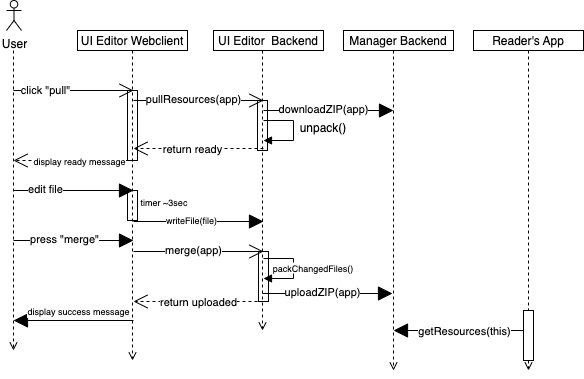
\includegraphics[width=\textwidth]{pics/user-flow.uml.drawio.png}